\section{Solution proposal}
In order to reflect the power of vision language models as high-level instruction orchestrators inside a robotic environment, I worked inside \textit{NVIDIA IsaacSim}. An open source SOTA framework for robotics simulation and synthetic data generation in physically based virtual environments built on top of \textit{NVIDIA Omniverse}. My final solution proposes a simulated robotic multi-agent environment where the vision language clearly dominates the high-level decision making, and orchestrates the whole workflow pipeline with the information received and sent to the other agents in the scenario. 



\section{System architecture}
Un esquema general de cómo se conectan el VLM, el simulador y los agentes (el "big picture"). 

% VLM will act as object identificator -> distinguishing them -> predicted coordinates

\section{Workflow}
The workflow used for the final scenarios inside \textit{IsaacSim} could be reduced to this basic pipeline, illustrated below. The following workflow stands for the "standard" pipeline, however, depending on the desired task components of the pipeline will follow different procedures or repeat their selves more than one time. 

\begin{enumerate}
	\item \textbf{Visual captioning}: there will be cameras distributed throughout the scenario, pointing towards the key interest points where the VLM must put into action its reasoning capabilities. A screenshot of the area will be taken and sent to the next step.
	
	\item \textbf{CV algorithms to enhance detection}: depending on the target object to be detected by the vision language model specified in the next component, a specific computer vision algorithm application script will be called. In order to modify the screenshot image so the specified target is more detectable. 
	
	\item \textbf{VLM hosted on BentoML}: there will be a \textit{BentoML} server running up ready to capture the CV-modified screenshot of the desired section of the scenario taken in the previous step. However, as VLM receive a pair of (image-text) as input, the image will be accompanied by a prompt. Prompt consisting of identifying a specific target inside the scenario area captured by the camera. While the service is running, another component will be responsible for coordinating the calls with the server's API.
	
	\item \textbf{Target object coordinates prediction}: another script will interact with the VLM to try to get the closest coordinate predictions of the target object. Passing the prediction through hallucination filters and other several functions to get the most reliable function. 
	
	\item \textbf{Movement synchronization}: after getting the predicted coordinates, a dynamic movement script will be executed to get to those position. Depending on the robot agent and the task objective, the movement will end in itself or serve as bridge to another movement later on.
\end{enumerate} 

Depending on the task, there could be just one target object detection and movement cycle, or more than one as in the case of multi-agent scenarios. 

%\begin{figure}[H]
%	\centering
%	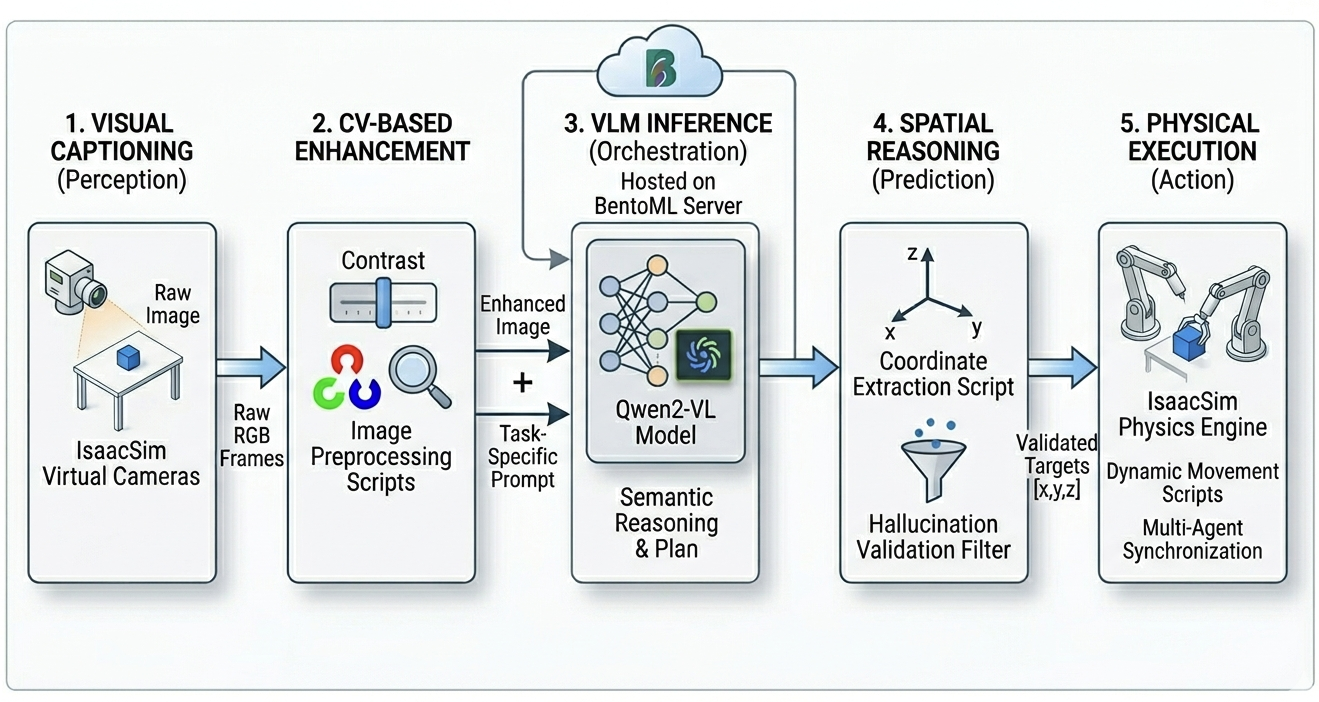
\includegraphics[width=.8\textwidth]{imgs/workflow.png}
%	\label{fig:workflow}
%	\caption{Standard workflow of the solution, going from the visual captioning stage up to the physical agent movement execution.}
%\end{figure}

\usetikzlibrary{arrows.meta, positioning, shapes.geometric}

\begin{figure}[h]
	\centering
	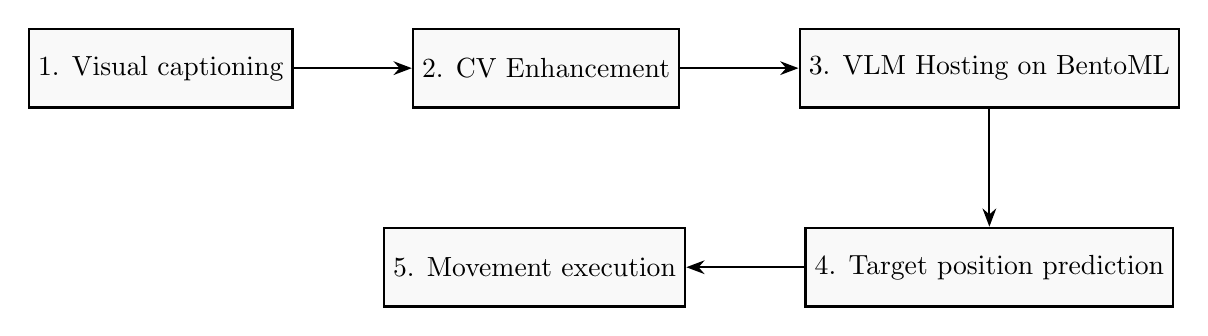
\begin{tikzpicture}[
		node distance=1.5cm,
		state/.style={rectangle, draw, minimum width=3cm, minimum height=1cm, text centered, line width=0.8pt, fill=gray!5}
		]
		% Nodes
		\node (p1) [state] {1. Visual captioning};
		\node (p2) [state, right=of p1] {2. CV Enhancement};
		\node (p3) [state, right=of p2] {3. VLM Hosting on BentoML};
		\node (p4) [state, below=of p3] {4. Target position prediction};
		\node (p5) [state, left=of p4] {5. Movement execution};
		
		% Arrows
		\draw [-Stealth, line width=0.8pt] (p1) -- (p2);
		\draw [-Stealth, line width=0.8pt] (p2) -- (p3);
		\draw [-Stealth, line width=0.8pt] (p3) -- (p4);
		\draw [-Stealth, line width=0.8pt] (p4) -- (p5);
		
	\end{tikzpicture}
	\caption{Standard workflow of the solution, going from the visual captioning stage up to the physical agent movement execution.}
	\label{fig:minimalist_workflow}
\end{figure}

\section{Tools used}
Nvidia IsaacSim, Omniverse, IsaacLab, ... VLM, ... BentoML

Justificación técnica de por qué elegiste Qwen2-VL, Isaac Sim y EAGERx frente a otras alternativas.

